\newcommand\rep{U}
\setlength\epigraphwidth{8.5cm}
\epigraph{Valiant's work has shown that, even if our universe hadn't been made of bosons and fermions, theoretical computer scientists would have had compelling reasons of their own to invent those particles or something equivalent to them.}{--- \textup{Scott Aaronson}}
%https://www.scottaaronson.com/blog/?p=570

%------------------------------------
\section{Overview}
%------------------------------------

Given two $2 \times 2$ unitary matrices $U^+$ and $U^-$ with the same determinant, or equivalently $U^{\pm} \in \gr{SU}{2}$, we define a \emph{matchgate} to be a two-qubit unitary operator of the form
\begin{align}\label{def:matchgate}
M(U^+,U^-) &=
\begin{pmatrix}
U^+_{11} & 0 & 0 & U^+_{12} \\
0 & U^-_{11} & U^-_{12} & 0 \\
0 & U^-_{21} & U^-_{22} & 0 \\
U^+_{21} & 0 & 0 & U^+_{22}
\end{pmatrix}.
\end{align}
When qubits are arranged in a one-dimensional array, nearest neighbor (N.N) matchgates form a restricted class of quantum operations.  Notice that because the operation $M(\id,X)$ that swaps a pair of qubits is not a matchgate, the N.N. constraint is non-trivial.  Via the Jordan-Wigner transformation, the matchgates can also be interpreted as the evolution of systems of non-interacting fermions, sometimes called \emph{fermionic linear optics}, as will be discussed in \autoref{ch5:matchgate}.

If the input state of an N.N. matchgate circuit is the computational basis state $\ket{0}^{\otimes n}$ and the only measurements made are the Pauli measurements $Z^{\otimes k}$ on any subset of $k\le n$ qubits, then the probability of a given outcome can be calculated in polynomial time on a classical computer \cite{valiant_quantum_2002}. Thus, a subtheory that consists of states that can be prepared from the computational basis state by a matchgate evolution and Pauli $Z$ measurements is qualified to be a classical subtheory. \autoref{ch5:classical-simulation} is a review of the classical simulatability of N.N. matchgates in the language of fermionic Gaussian states and the relation between matchgates and universal quantum computation.

After a brief discussion of existing approaches to fermionic phase space in \autoref{ch5:phase-space}, we introduce some properties of the spinor representations in \autoref{ch5:spinor} to prepare the reader for our construction of the Stratonovich-Weyl (SW) phase spaces (\autoref{ch3:SW}). We then show in \autoref{ch5:four-modes} that despite the classicality of the Gaussian states, their quasi-probability functions in the $\gr{SO}{2n}$-covariant analogue of the Wigner function may not be positive. We do so by explicitly constructing the quasi-probability representation in the first nontrivial case, the four-mode case, and calculate the integrated negativity of the Gaussian quasi-probability functions.

%------------------------------------
\section{Fermionic linear optics}\label{ch5:FLO}
%------------------------------------

As we all know, the Hilbert space of $k$ indistinguishable fermions is the anti-sym\-me\-tric subspace $\bwedge^k \hilb \subset \bigotimes^k \hilb$ spanned by
\begin{align}
\psi_1 \wedge \cdots \wedge \psi_k &\coloneqq
\frac{1}{\sqrt{k!}} \sum_{\sigma \in S_k} \text{sgn} \sigma\,
\psi_{\sigma(j)} \cdots \psi_{\sigma(j)},
\end{align}
where $\psi_{j} \in \hilb$ and the sum is over all permutations $\sigma$ with $\text{sgn}\, \sigma = +1$ if $\sigma$ is even and $\text{sgn}\, \sigma = -1$ if $\sigma$ is odd. The $n$-mode \emph{fermionic Fock space} is the direct sum of the $k$-fermion sectors
\begin{align}
\hilb_{\text{Fock}}(n) &= \bigoplus_{k=0}^n \bwedge^k \hilb,
\end{align}
where $\bwedge^0 \hilb$ is the zero-fermion sector --- the designated \emph{vacuum state} $\ket{0\cdots 0}$.
Also of physical significance are the even and odd parity subspaces
\begin{align}
\hilb^+_{\text{Fock}}(n) &= \bigoplus_{0\le 2k \le n} \bwedge^{2k} \hilb, &
\hilb^-_{\text{Fock}}(n) &= \bigoplus_{1\le 2k+1 \le n} \bwedge^{2k+1} \hilb.
\end{align}
The parity superselection rule forbids any superposition of states in $\hilb^+_{\text{Fock}}(n)$ and $\hilb^-_{\text{Fock}}(n)$. $\hilb_{\text{Fock}}(n)$ has the dimension $\sum_{k=0}^n {n \choose k} = 2^n$ while $\hilb^{\pm}_{\text{Fock}}(n)$ have the dimension $2^{n-1}$. An orthonormal basis for $\hilb_{\text{Fock}}(n)$ can be built from the vacuum by applying creation operators\footnote{A detailed derivation can be found in \cite{nielsen2005fermionic}.}
\begin{align}
\ket{x_1 \cdots x_n} &= (a_1\dgg)^{x_1} \cdots (a_n\dgg)^{x_n} \ket{0\cdots 0},
\end{align}
where $a_j$ and $a_j\dgg$ obey the canonical anti-commutation relations
\begin{align}
&\{a_j,a_k\dgg\} = \delta_{jk}\id,
&\{a_j,a_k\} = 0.
\end{align}
These states are eigenstates of the number operator $N_j = a\dgg_j a_j$ for each mode $j$,
\begin{align}
	N_j \ket{x_1 \cdots x_n} &= x_j\ket{x_1 \cdots x_n}.
\end{align}
The action of the creation and annihilation operators on these number states consistent with the anti-commutation relations is given by
\begin{align}
	\begin{split}\label{pre-jordan-wigner}
		a\dgg_j \ket{x_1 \cdots x_n} &= (-1)^{\sum_{k=1}^{j-1} N_k} \delta_{x_j,0} \ket{x_1 \cdots x_{j-1}\, 1\, x_{j+1} \cdots x_n}, \\
		a_j \ket{x_1 \cdots x_n} &= (-1)^{\sum_{k=1}^{j-1} N_k} \delta_{x_j,1} \ket{x_1 \cdots x_{j-1}\, 0\, x_{j+1} \cdots x_n},
	\end{split}
\end{align}
where $\sum_{k=1}^{j-1} N_k$ counts the number of fermions in the first $j-1$ modes.

It is useful to introduce $2n$ Hermitian \emph{majorana operators}:
\begin{align}
c_{2j-1} &\coloneqq a_j + a_j\dgg, &
c_{2j}&\coloneqq \frac{a_j - a_j\dgg}{i}, &
a_j &= \frac{c_{2j-1} + ic_{2j}}{2},
\end{align}
satisfying the defining anti-commutation relations of the $2n$-dimensional \emph{Clifford algebra}\footnote{If the Euclidean metric $\delta_{jk}$ is replaced by the Minkowski metric $\eta_{jk}$, they are known as \emph{Dirac's gamma matrices}, in fermionic quantum field theories \cite{Peskin}. One can start with the Clifford algebra and derive the properties of spinor representations of spin groups \cite{FH}.}
\begin{align}
\{c_j,c_k\} &= 2\delta_{jk}\id.
\end{align}
Let $\mathcal{C}_1$ be the span of all majorana operators $\{c_j\}$ and $\mathcal{C}_2$ be the span of all quadratic products $\{c_jc_k|j \neq k\}$. (The identity operator generating a global phase is irrelevant to the computation.) $\mathcal{C}_2$ is isomorphic to the Lie algebra $\al{so}(2n)$ where the isomorphism is given by defining Hermitian operators $J_{jk} \coloneqq i[c_j,c_k]/4$. We have
\begin{align}
J_{jk}\dgg &= -J_{kj}, \\
[c_j,J_{kl}] &= i(\delta_{jk}c_l - \delta_{jl}c_k), \label{adjoint-commutation-relation} \\
[J_{jk},J_{lm}] &= -i(\delta_{jl}J_{km} - \delta_{kl}J_{jm} + \delta_{km}J_{jl} - \delta_{jm}J_{kl}).
\label{so(n)-commutation-relation}
\end{align}
Thus the Fock space
$\hilb_{\text{Fock}}(n)$ is a representation of $\al{so}(2n)$ generated by quadratic Hamiltonians of the form
\begin{align}\label{quadratic-hamiltonian}
H &= \sum_{\substack{j,k \\ j<k}} h_{jk} J_{jk}
= \frac{i}{4} \sum_{\substack{j,k \\ j<k}} h_{jk} [c_j,c_k],
\end{align}
where $h_{jk}$ is an arbitrary real anti-symmetric matrix.

We define \emph{Fermionic linear optics} to be the set of unitary operators that transform every element of $\mathcal{C}_1$ linearly by conjugation. In other words, if we stack $2n$ majorana operators into a vector
\begin{align}
	{\bf c}^T &= \begin{pmatrix}
		c_1 \cdots c_{2n}
	\end{pmatrix},
\end{align}
and write
\begin{align}
	c_j(t) &= U\dgg(t) c_j U(t),
\end{align}
then there is some $2n$-by-$2n$ matrix $R$ such that
\begin{align}
	{\bf c}(t) &= R {\bf c}(0).
\end{align}
In fact, $R$ must be an orthogonal matrix to preserve the anti-commutation relation.
\begin{theorem}
Fermionic linear optics is exactly the set of evolutions by quadratic Hamiltonians $H = \sum_{\substack{j,k \\ j<k}} h_{jk} J_{jk}$.
\end{theorem}\label{thm:adjoint-action}
\begin{proof}
	Consider
	\begin{align}
		\frac{dc_j(t)}{dt}
			&= \frac{d}{dt}\left(e^{-iHt} c_j e^{iHt}\right) = i[c_j(t),H].
	\end{align}
	Using the commutation relation \eqref{adjoint-commutation-relation} between $c_j$ and $J_{jk}$ and the fact that $H$ commutes with $e^{iHt}$, we obtain the differential equation
	\begin{align}
		\frac{dc_j(t)}{dt} &= h_{jk} c_j(t),
	\end{align}
	whose solution is
	\begin{align}
		{\bf c}(t) &= e^{ht} {\bf c}(0).
	\end{align}
	Since $h$ is an arbitrary real anti-symmetric matrix, the vector space $\mathcal{C}_1$ is isomorphic to the defining representation of the real orthogonal group $\gr{SO}{2n}$ (\autoref{ch2:matrix-group}) and the theorem is proved.
\end{proof}

%------------------------------------
%\subsection{็Fermionic linear optics}\label{ch5:FLO}
%------------------------------------

%What is the operational theory we are trying to represent as quasi-probabilities here? To apply the formalism from the last chapter, we need the Hilbert space $\hilb$ to be a unitary reducible representation of a Lie group $G$ and we need a fiducial state $\ket{e} \in \hilb$. The dual frame is a natural choice since we are interested in the negativity of the quasi-probability functions of both states and measurements. Moreover, in quantum computation, the fiducial state and the fiducial measurement are often assumed to be symmetric: the state is prepared and measured in the computational basis state $\ket{0}^{\otimes n}$. (The measurement corresponds to the Pauli $Z^{\otimes n}$ measurement.) Having made the choice, what determines the subtheory is really then the dynamics, which is provided by the Lie group $G$.


%------------------------------------
\subsection{Jordan-Wigner transformation and matchgates}\label{ch5:matchgate}
%------------------------------------

The fact that $\hilb_{\text{Fock}}(n)$ is isomorphic to $\mathbb{C}^{2^n}$ as a vector space suggests that we identify the fermionic Fock space with a system of $n$ qubits. What should be the action of the fermionic operators in the multi-qubit space? If we identity the number states with the computational basis states for $n$ qubits in the obvious way, eq. \eqref{pre-jordan-wigner} tells us that
\begin{align}
a_j = \left( \bigotimes_{k=1}^{j-1} Z \right) \otimes  \ket{0}_j\!\bra{1},
\end{align}
gives an isomorphism. This isomorphism, known as the \emph{Jordan-Wigner transformation}, is in fact the smallest irrep of the canonical anti-commutation relation ---the fermionic analogue of the Stone-von Neumann theorem for canonical commutation relations \cite{Derezinski}. The transformation allows one to map between a system of fermions and a system of qubits (spin-1/2 system) and has been employed, for example, to solve the problem of simulating interacting fermions on a quantum computer \cite{ortiz_quantum_2001}, posed by Feynman since the inception of the idea of quantum computation \cite{feynman_simulating_1982}.

Under the Jordan-Wigner transformation, majorana operators correspond to the multi-qubit Pauli operators
\begin{align}
c_{2j-1} &= \bigotimes_{k=1}^{j-1} Z_k \otimes X_j, &
c_{2j} &= \bigotimes_{k=1}^{j-1} Z_k \otimes Y_j.
\end{align}
%All $J_{jk}$ for $j<k$ have the form
%\begin{align}
%	J_{jk} &= \pm i U_j \otimes Z_{j+1} \otimes\cdots\otimes Z_{k-1} V_k,
%\end{align}
%where $U$ and $V$ is $X$ or $Y$.
The Jordan-Wigner transformation is very non-local as typical quadratic operators in $\mathcal{C}_2$ are, for instance, of the form
\begin{align}
	\pm i\sigma_j Z_{j+1} \cdots Z_{k-1}\sigma_k,
\end{align}
where the $\sigma$ are $X$ or $Y$.
But certain products remain local in both the fermion and the qubit pictures:
\begin{equation*}
\noindent\begin{minipage}[t]{.5\textwidth}
\begin{align}
c_{2j} c_{2j+1} &= iX_j X_{j+1}, \\
c_{2j-1} c_{2j+2} &= -iY_j Y_{j+1}, \\
c_{2j-1} c_{2j} &= iZ_j,
\end{align}
\end{minipage}
\begin{minipage}[t]{.5\textwidth}
\begin{align}
c_{2j-1} c_{2j+1} &= -i Y_j X_{j+1}, \\
c_{2j} c_{2j+2} &= iX_j Y_{j+1}.
\end{align}
\end{minipage} \nonumber
\end{equation*}
Such local products are precisely the infinitesimal generators of N.N. matchgates,
\begin{align}
	X^{\pm} &= \frac{1}{2i} (c_{2j} c_{2j+1} \pm c_{2j-1} c_{2j+2}) = \frac{X_j X_{j+1} \mp Y_j Y_{j+1}}{2}, \\
    Y^{\pm} &= \frac{i}{2} (c_{2j-1} c_{2j+1} \mp c_{2j} c_{2j+2}) = \frac{Y_j X_{j+1} \pm X_j Y_{j+1}}{2}, \\
    Z^{\pm} &= \frac{1}{2i} (c_{2j-1} c_{2j} \pm c_{2j+1} c_{2j+2}) = \frac{Z_j \pm Z_{j+1}}{2},
\end{align}
and these are the Pauli matrices in the even and odd parity subspace that infinitesimally generate the $U^{\pm} \in \gr{SU}{2}$ in N.N. matchgates \eqref{def:matchgate}.

What about quadratic majorana operators that are mapped to operators on three or more qubits? Non-nearest neighbor matchgates are mapped to quartic and higher order majorana operators by the Jordan-Wigner transformation. But it turns out that such operators are not needed in order to implement fermionic linear optics if we are willing to accept a polynomial overhead in the number of N.N. matchgates. More specifically, an arbitrary $\gr{SO}{2n}$ rotation can be broken up into $\mathcal{O}(n^2)$ elementary rotations, each of which is nontrivial on only two fermionic modes \cite{hoffman_generalization_1972}. Then $\mathcal{O}(n)$ N.N. matchgates of the form
\begin{align}\label{def:modal-swap}
	M_j(Z,X) = \frac{1}{2i}(c_{2j}c_{2j+1} - c_{2j-1}c_{2j+2} + c_{2j-1}c_{2j} + c_{2j+1}c_{2j+2})
	&= \begin{pmatrix}
		1 & 0 & 0 & 0 \\
		0 & 0 & 1 & 0 \\
		0 & 1 & 0 & 0 \\
		0 & 0 & 0 & -1
	\end{pmatrix}
\end{align}
can be applied to swap the modes
\begin{align}
	M\dgg_j(Z,X) c_{2j-1} M_j(Z,X) &= c_{2j+1}, & M\dgg_j(Z,X) c_{2j} M_j(Z,X) &= c_{2j+2},
\end{align}
bringing each elementary rotation to a N.N. matchgate, giving a total $\mathcal{O}(n^3)$ overhead.

Matchgates were originally introduced by Valiant \cite{valiant_quantum_2002,valiant_holographic_2008} for the purpose of studying algorithms for graphs. A \emph{perfect matching} of a graph $G$ is a set $M$ of edges in $G$ such that each vertex in $G$ connects to exactly one edge in $M$. The problem of counting the number of perfect matchings for a general graph is very hard. More precisely, counting perfect matchings is equivalent to computing the permanent of the adjacency matrix for the graph. The \emph{permanent} of an $n$-by-$n$ matrix is similar to the determinant except that there is no alternating sign:
\begin{align}
	\text{Per} A &= \sum_{\sigma \in S_n} \prod_{j=1}^n a_{j\sigma{j}}.
\end{align}
For general matrices (even if the entries are only 0 or 1), the problem was proved by Valiant to be \#P-complete \cite{valiant_complexity_1979}.\footnote{Perfect matching was the first problem found for which the decision version: ``is there a perfect matching?" can be answered in polynomial time while the counting version ``how many perfect matchings are there?" is in \#P~\cite{AB}.} For planar graphs however, the problem reduces to computing the \emph{Pfaffian} of the adjacency matrix\footnote{The Pfaffian is only defined for anti-symmetric matrices. So it is actually the Pfaffian of the \emph{directed} adjacency matrix that corresponds to the number of perfect matchings.} and can be solved in polynomial time by the Fisher-Kasteleyn-Temperley (FKT) algorithm \cite{kasteleyn_statistics_1961,temperley_dimer_1961,kasteleyn_dimer_1963}.  

Fix $n$ vertices of $G$ to be ``input" vertices, labeled by $j_1 \dots j_n$. Likewise, fix $m$ vertices of $G$ to be ``outputs", labeled by $k_1 \dots k_n$. A family of graphs  $G^{j_1 \dots j_n}_{k_1 \dots k_n}$, where each $j$ or $k$ takes a binary value, is obtained from $G$ by erasing the input and output vertices with $j$ or $k=1$. Let $\mathcal{M}(G)$ be the set of perfect matchings for a weighted planar graph $G$ with edges $(j,k)$ of weight $w_{jk}$. The tensor components
\begin{align}\label{match-sum}
M^{j_1 \dots j_n}_{k_1 \dots k_n} &= \sum_{M \in \mathcal{M}\left( G^{j_1 \dots j_n}_{k_1 \dots k_n} \right)} \prod_{(jk) \in M} w_{jk},
\end{align}
can also be computed in polynomial time by the FKT algorithm. Valiant defined matchgates to be these tensors with some technical restrictions such that a circuit composed of matchgates corresponds to a contraction of matchgate tensors that computes the sum \eqref{match-sum} of a certain graph related to $G$ in polynomial time. Matchgates as defined by Valiant are not necessarily invertible or even square, but he observed that when they are unitary as in our definition \eqref{def:matchgate}, his algorithm gives a classical polynomial-time algorithm to simulate a class of quantum circuits.

%------------------------------------
\subsection{Fermionic Gaussian states}\label{ch5:gaussian}
%------------------------------------

Any operator $A$ that can be written as a linear combination of products of an even number of majorana operators is said to be an \emph{even operator}:
\begin{align}
	A &= \alpha_0 \id + \alpha_{j_1j_2} c_{j_1} c_{j_2} + \cdots + \alpha_{1,\dots,2n} c_1 \cdots c_{2n}.
\end{align}
A \emph{fermionic Gaussian state} $\rho$ is an even state characterized by the following equivalent properties:\footnote{Strictly speaking, what we define here are fermionic Gaussian states in the even or odd spinor representation. Mathematical properties of general fermionic Gaussian states without the parity superselection rule are discussed in \cite{oeckl_coherent_2015}.}
\begin{enumerate}
	\item $\rho$ can be expressed in the form
	\begin{align}\label{def:fermion-gaussian-state}
		\rho &= N \exp\!\Bigg(-\frac{i}{2}\sum_{\substack{j,k \\ j<k}} \beta_{jk} c_jc_k\Bigg),
	\end{align}
	where $\beta_{jk}$ is a real anti-symmetric matrix and $N$ is the normalization constant. ($\rho$ that is not full-rank is obtained by setting some $\beta_{jk}$, the ``inverse temperature", to $\infty$.)
	\item For $m<n$, the $2m$-order correlation function can be obtained from the real anti-symmetric \emph{correlation matrix}
	\begin{align}\label{def:correlation-matrix}
		\Sigma_{jk} = \frac{i}{2} \Tr (\rho [c_j,c_k])
	\end{align}
	by \emph{Wick's theorem}:
	\begin{align}\label{thm:wick}
		\Tr (\rho c_{j_1} \cdots c_{j_{2m}}) &= \frac{1}{i^m} \text{Pf}\left( \Sigma\bigr|_{j_1 \cdots j_{2m}} \right),
	\end{align}
	where Pf is the Pfaffian of an anti-symmetric matrix
	\begin{align}
		\text{Pf}^2 A &= \det A,
	\end{align}
	and $\Sigma\bigr|_{j_1 \cdots j_{2m}}$ is the submatrix of $\Sigma$ containing only the entries $(j,k)$ in the range $\{ j_1,\dots,j_{2m} \}$. A proof of Wick's theorem can be found in standard quantum field theory references such as \cite{Peskin}. The theorem in terms of the Pfaffian is described in \cite{terhal_classical_2002} and references therein.
	\item Fermionic Gaussian states are the orbit of the product state $N \exp(\sum_j \beta_j N_j)$ under the spin group $\gr{SO}{2n}$. In particular, pure fermionic Gaussian states are the orbit of the state $\ket{0}^{\otimes n}$.
\end{enumerate}
Every fermionic Gaussian state can be brought to the canonical form
\begin{align}
	\rho &= \frac{1}{2^n} (\id + i\lambda_1 \tilde{c}_1 \tilde{c}_2) \cdots (\id + i\lambda_{n} \tilde{c}_{2n-1} \tilde{c}_{2n}),
\end{align}
where $\{ \tilde{c}_j \}$ obey the anti-commutation relation for the majorana operators, by the following theorem.\footnote{The theorem also follows from the fact that every element of a semisimple Lie algebra is conjugated to an element in the Cartan subalgebra, which for $\al{so}(2n)$ has the block-diagonal form \eqref{block-diagonal-form}.}

\begin{theorem}
Any real anti-symmetric matrix $\beta$ can be brought into the block-diagonal form
\begin{align}\label{block-diagonal-form}
R\beta R^T = \bigoplus_{j=1}^n \left( \begin{array}{cc} 0 & \beta_j \\ -\beta_j & 0 \end{array} \right),
\end{align}
by a rotation $R \in SO(2n)$.
\end{theorem}
\begin{proof}
	First, since $\beta$ is real and anti-symmetric, $i\beta$ is Hermitian. Moreover, $\beta$ and its transpose $\beta^T = -\beta$ have the same eigenvalues. So we conclude that eigenvalues of $\beta$ must be purely imaginary and occur in pairs $\pm i\beta_j$, where each $\beta_j$ is real.
	We want to show that $\beta$ can be brought into the block-diagonal form
	\begin{align}
		\bigoplus_{j=1}^n \begin{pmatrix}
			0 & -\beta_j \\
			\beta_j & 0
		\end{pmatrix}
	\end{align}
	by an $\gr{SO}{2n}$ rotation. Geometrically, this says that any rotation in $2n$ dimensions is a product of independent rotations on $n$ orthogonal planes. Following \cite[Appendix D.4]{dreiner_two-component_2010}, consider the positive semidefinite matrix $\beta^T\beta$ having real eigenvectors $\{ \ket{w_j}, \ket{u_j} \}$:
	\begin{align}
		\beta^T\beta \ket{w_j} &= 0 & \beta^T\beta \ket{u_j} &= \beta_j^2 \ket{u_j}.
	\end{align}
	Note that $\{ \ket{w_j}\}$ are exactly the eigenvectors of $\beta$ with eigenvalue zero because $\braket{w_j| \beta^T\beta |w_j} = 0$ implies that $\beta\ket{w_j} = 0$. If we define
	\begin{align}
		\ket{v_j} &= \frac{\beta}{\beta_j} \ket{u_j},
	\end{align}
	then $\ket{v_j}$ is orthogonal to $\ket{u_j}$ by the anti-symmetry:
	\begin{align}
		\braket{u_j|v_j} &= \frac{1}{\beta_j} \braket{u_j|\beta|u_j} =0.
	\end{align}
	So we have a $2n$-by-$2n$ orthogonal matrix
	\begin{align}
		R &= \begin{pmatrix}
			v_1 & u_1 & \cdots & v_{n-k/2} & u_{n-k/2} & w_1 & \cdots & w_k
		\end{pmatrix}
	\end{align}
	that brings $\beta$ into the block-diagonal form
	\begin{align}
		R \beta R^T &= \bigoplus_{j=1}^n \begin{pmatrix}
				0 & -\beta_j \\
				\beta_j & 0
			\end{pmatrix}
	\end{align}
	as desired.
\end{proof}
\noindent In the canonical form, eq. \eqref{def:fermion-gaussian-state} has the form
\begin{align}
\rho &= N\exp \left( -\frac{i}{2} \sum_{j=1}^n \beta_j \tilde{c}_{2j-1} \tilde{c}_{2j} \right)
= N\prod_{j=1}^n \exp \left[ \frac{\beta_j}{2} (-i\tilde{c}_{2j-1} \tilde{c}_{2j}) \right].
\end{align}
The exponential factorizes since quadratic majorana operators commute if they do not share a common majorana operator. Expanding the exponential in a Taylor series,
\begin{align}
\rho & = N\prod_{j=1}^n \left[ \id + \frac{\beta_j}{2} (-i\tilde{c}_{2j-1} \tilde{c}_{2j}) + \frac{1}{2!} \left( \frac{\beta_j}{2} \right)^2 (-i\tilde{c}_{2j-1} \tilde{c}_{2j})^2 + \cdots \right] \nonumber \\
& = N\prod_{j=1}^n \left[ \sum_{m=0}^{\infty} \frac{1}{(2m)!} \left( \frac{\beta_j}{2} \right)^{2m} \id +\sum_{m=0}^{\infty} \frac{1}{(2m+1)!} \left( \frac{\beta_j}{2} \right)^{2m+1} (-i\tilde{c}_{2j-1} \tilde{c}_{2j})  \right] \nonumber \\
& = N\prod_{j=1}^n \left[ \cosh \frac{\beta_j}{2} \id + \sinh \frac{\beta_j}{2} (-i\tilde{c}_{2j-1} \tilde{c}_{2j}) \right] \nonumber \\
& = \left( N\prod_{j=1}^n \cosh \frac{\beta_j}{2} \right) \prod_{j=1}^n \left[ \id + \tanh \frac{\beta_j}{2} (-i\tilde{c}_{2j-1} \tilde{c}_{2j}) \right] \nonumber \\
& = \frac{1}{2^n} \prod_{j=1}^n ( \id - i \lambda_j \tilde{c}_{2j-1} \tilde{c}_{2j} ),
\end{align}
where $\lambda_j \coloneqq \tanh (\beta_j/2)$. This induces the canonical form of the correlation matrix
\begin{align}
	\widetilde\Sigma_{2j-1,2j} &= i \Tr \left[ \rho \tilde{c}_{2j-1} \tilde{c}_{2j} \right] \nonumber \\
		&= \frac{i}{2^n} \Tr \left[ \prod_{k=1}^n (\id - i\lambda_j \tilde{c}_{2k-1} \tilde{c}_{2k}) \tilde{c}_{2j-1} \tilde{c}_{2j} \right] \nonumber \\
		&= \frac{i}{2^n} \Tr \left[ \prod_{k\neq j}^n (\id - i\lambda_j \tilde{c}_{2k-1} \tilde{c}_{2k}) (\tilde{c}_{2j-1}\tilde{c}_{2j} + i\lambda_j \id) \right] = -\lambda_j,
\end{align}
where we have used the fact that every product of majorana operators except $\id$ is traceless.
Thus, we have
\begin{align}
	\widetilde\Sigma &=
		\bigoplus_{j=1}^n \left( \begin{array}{cc} 0 & -\lambda_j \\ \lambda_j & 0 \end{array} \right)
\end{align}
with coefficients $\lambda_j$ having values $-1\le \lambda_j \le 1$ so that
\begin{align}
	\Sigma^T \Sigma &< \id.
\end{align}
For pure states, each $\lambda_j$ is either $+1$ or $-1$. The computational basis state $\ket{0}^{\otimes n}$, for example, is a Gaussian state having the correlation matrix with $\lambda_j =1$ for all $j$. In fact, it is well known that all number states are Gaussian states, in striking contrast to the usual boson number states.

%------------------------------------
\subsection{Classical simulatability and approaches to universality}\label{ch5:classical-simulation}
%------------------------------------

The classical simulatability of fermionic linear optics readily follows from the properties of fermionic Gaussian states.
\begin{enumerate}
	\item The description of a Fermionic Gaussian state is encoded in its correlation matrix \eqref{def:correlation-matrix}, with $\mathcal{O}(n^2)$ elements.
	\item Fermionic linear optics preserves Gaussianity and induces a rotation on the vector space of linear majorana operators $\mathcal{C}_1$ (Theorem \ref{thm:adjoint-action}), which can be broken up into $\mathcal{O}(n^3)$ N.N. matchgates, and the correlation matrix can be updated in polynomial time.\footnote{In fact, the adjoint action of a Lie group $G$ on its Lie algebra $\al{g}$ can be computed in time that is polynomial in the dimension of $\al{g}$ and digits of accuracy \cite{somma_efficient_2006,jozsa_jordan-wigner_2015}.}
	\item The probability of a given outcome of the number measurements (or equivalently the Pauli $Z$ measurements) on any subset of $k<n$ modes can be evaluated by Wick's theorem \eqref{thm:wick}. In particular, the Pfaffian (or the determinant) can be calculated in $\mathcal{O}(n^3)$ time by Gaussian elimination.
\end{enumerate}

Moreover, number measurements project Gaussian states onto Gaussian states.
In spite of the famous sign problem in numerically simulating systems of interacting fermions, the computational power of fermionic linear optics is decidedly weaker than that of its bosonic counterpart. Whereas bosonic linear optics become universal for quantum computation when supplemented with adaptive measurements \cite{knill_scheme_2001} and the distribution of photons under linear optical operations is proved to be hard to simulate classically based on plausible complexity-theoretic conjectures \cite{aaronson_computational_2011}, adaptive measurements have no effect on the computational power of fermionic linear optics \cite{terhal_classical_2002} and fermion number states are Gaussian as noted before. Matchgates are also shown to be computationally equivalent to space-bounded quantum computation \cite{jozsa_matchgate_2010} and the so-called linear threshold gates \cite{nest_quantum_2011}.

Classical simulatability of matchgates has been extended to classical simulatability of matchgates ``intertwined" with Clifford operations (the operations preserving the Pauli group introduced in \autoref{ch4:discrete-wigner}) \cite{jozsa_matchgates_2008}, to non-invertible matchgates \cite{knill_fermionic_2001,jozsa_jordan-wigner_2015}, and recently to matchgates preceded or followed by arbitrary single-qubit rotations \cite{brod_efficient_2016}. Interestingly, including unitary operations that are exponentials of linear majorana operators
\begin{align}
c_{2j-1} &= \bigotimes_{k=1}^{j-1} Z_k \otimes X_j, &
c_{2j} &= \bigotimes_{k=1}^{j-1} Z_k \otimes Y_j,
\end{align}
which is equivalent to extending $\gr{Spin}{2n}$ to $\gr{Spin}{2n+1}$, also adds the ability to precede matchgates by arbitrary single-qubit rotations because the string of Pauli $Z$'s acts trivially on the input state $\ket{0}^{\otimes n}$. We can also turn the exponentials of linear majorana operators to single-qubit rotations on the first qubit at any stage in the computation by the modal swap matchgate \eqref{def:modal-swap}, recovering another classical simulatability result in \cite{jozsa_jordan-wigner_2015}.

One can ask the question: why are N.N. matchgates non-universal? It is well known that the ability to perform arbitrary single-qubit rotations and an entangled operation suffices for universal quantum computation. N.N. matchgates can generate the Bell state $(\ket{00} + \ket{11})/\sqrt{2}$, so clearly they are capable of entangling qubits. Therefore, they must lack single-qubit rotations. However, if one encodes one logical qubit into two qubits
\begin{align}
	\ket{0}_L &= \ket{00}, & \ket{1}_L &= \ket{11},
\end{align}
then matchgates of the form $M(U^+,U^+)$ can perform arbitrary single-logical-qubit rotations, so N.N. matchgates must lack logical entangling operations \cite{brod_extending_2011}. In fact, every parity-preserving unitary operation that is not a matchgate (that is, $M(U^+,U^-)$ without the determinantal constraint $\det U^+ = \det U^-$) is entangling in this encoding.

Approaches to universality for quantum computation have been considered both from the viewpoints of fermionic linear optics and matchgate computation. Fermionic linear optics becomes universal if supplemented by a quartic interaction \cite{bravyi_fermionic_2002} or a quartic measurement \cite{bravyi_fermionic_2002,beenakker_charge_2004} such as $-c_{2j-1}c_{2j}c_{2k-1}c_{2k} = Z_jZ_k$. An addition of next-nearest-neighbor matchgates or, equivalently, the swap operation
\begin{align}
	\begin{pmatrix}
		1 & 0 & 0 & 0 \\
		0 & 0 & 1 & 0 \\
		0 & 1 & 0 & 0 \\
		0 & 0 & 0 & 1
	\end{pmatrix},
\end{align}
which itself is not a matchgate, also suffices to promote N.N. matchgates to universality \cite{jozsa_matchgates_2008}. All of these are consistent with earlier results on quantum computation by the anisotropic Heisenberg interaction $H_H$ and the isotropic exchange interaction $H_E$ \cite{divincenzo_universal_2000,kempe_encoded_2001,kempe_exact_2002}:
\begin{align}
	H_H &= X_jX_k + Y_jY_k, \\
	H_E &= X_jX_k + Y_jY_k + Z_jZ_k.
\end{align}
$H_H$ interactions generate matchgates, and they become universal if the interaction is not limited only to nearest neighbor spins, whereas $H_E$ includes quartic interactions and is universal.

A different approach to universality is based on resource states such as the eight-majorana-fermion state introduced in \cite{bravyi_universal_2006}
\begin{align}
	\ket{a_8} &= \frac{\ket{0000}+\ket{1111}}{\sqrt{2}},
\end{align}
which cannot be created by N.N. matchgates. The approach is analogous to gate injection via magic states in stabilizer computation \cite{bravyi_universal_2005}. Of particular importance to this protocol is the ability to distill the depolarized state
\begin{align}
	(1-p)\ketbra{a_8}{a_8} + p\frac{\id}{16}
\end{align}
into a state useful for universal quantum computation by fermions. \cite{bravyi_universal_2006} showed that this can be done for $p<0.4$. Later, \cite{melo_power_2013} together with \cite{oszmaniec_classical_2014} gave a range of $p \in \left[ 8/15, 8/11 \right]$ below which the resource state is distillable and above which the state becomes a convex combination of Gaussian states. For $p \in \left[ 8/15, 8/11 \right]$, it is not known whether the scheme in \cite{bravyi_universal_2006} is classically simulatable, quantum-computationally universal, or neither.


%------------------------------------
%\subsection{็All even two- and three-qubit pure states are Gaussian}\label{ch5:2-and-3-qubits}
%------------------------------------

 %Let us provide an alternative proof of this latter fact.
%\begin{theorem}
%	All even three-qubit pure states are fermionic Gaussian states.
%\end{theorem}
%\begin{proof}
%	The theorem can be proved in two steps. First, we establish the equivalence between the manifold of three-qubit fermionic Gaussian states $\homsp{SO}{6}{U}{3}$ and $\homsp{SO}{5}{U}{2}$, the orbit of the two-qubit computational basis state under the $\gr{SO}{5}$-action. Then we show that $\homsp{SO}{5}{U}{2}$ is the manifold of all two-qubit pure states, which coincides with the manifold of three-qubit even pure states ---they are both the complex projective space $\mathbb{C}P^3$.
%	
%	For the first step, we prove a stronger statement that $\homsp{SO}{2n+2}{U}{n+1} \simeq \homsp{SO}{2n+1}{U}{n}$ for all $n$ \cite{geiges2008introduction}. Every element of $\gr{SO}{2n+2}$ can be written uniquely as a product $su$ of $s \in \gr{SO}{2n+1}$ and $u \in \gr{U}{n+1}$.
%	\begin{itemize}
%		\item \emph{Existence} -- Both $\gr{SO}{2n+2}$ and $\gr{U}{n+1}$ have a transitive action on the $2n+1$-sphere. The former is obvious because the sphere is the homogeneous space$\homsp{SO}{2n+2}{SO}{2n+1}$. The latter is because matrices in $\gr{U}{n+1}$ are both orthogonal and symplectic. So it has the form
%			\begin{align}
%				U &= \begin{pmatrix}
%					A & -B \\
%					B & A
%				\end{pmatrix}
%			\end{align}, where
%		\item \emph{Uniqueness} --
%	\end{itemize}
%	As a result
%
%	 The quotient $X = SO(2n+2)/U(n+1) = SO(2n+1)\cdot U(n+1) /
%	    U(n+1)$ can be thought of as $ SO(2n+1)/U(n)$ because the
%	    $SO(2n+1)$-action on $X$ is transitive and the stabilizer of the identity
%	    $eU(n+1)$ of $X$ are the elements of $SO(2n+1)$ that are also in
%	    $U(n+1)$: $SO(2n+1) \cap U(n+1) = U(n)$.
%	
%	
%	 Observe that the manifold of $n$-qubit pure states and the manifold of $n+1$-qubit \emph{even} pure states coincide --- they are both the complex projective space $\mathbb{C}P^{2^n-1}$.
%	 \begin{align}
%	 	\homsp{SO}{6}{U}{3} \simeq \homsp{SO}{5}{U}{2} \simeq \mathbb{C}P^3.
%	 \end{align}
%	  So we only need to show that every two-qubit pure state can be reached from the computational basis state by some matchgate \emph{and} the exponential of some linear majorana operator. What the latter adds is the ability to perform an arbitrary single-qubit rotation before any matchgate.
%\end{proof}

% Since then, their computational capability has been further characterized \cite{jozsa_matchgate_2010,nest_quantum_2011,brod_extending_2011} and schemes for their classical simulation have been extended
%
% and extended by many authors \cite{jozsa_matchgate_2010,brod_extending_2011,brod_efficient_2016} and their relation to the Jordan-Wigner transformation clarified \cite{jozsa_matchgates_2008,jozsa_jordan-wigner_2015}.
%Matchgates are interesting for several reasons.
%\begin{enumerate}
%	\item The computational power of matchgates strongly depends on the connectivity of the qubits. Quantum circuits composed only of nearest neighbor (N.N.) matchgates are classically simulatable, whereas quantum circuits composed of arbitrary matchgates are universal as a quantum computer. This fact has been observed in the context of exchange interaction before \cite{divincenzo_universal_2000,kempe_encoded_2001,kempe_exact_2002}.
%	\item On the one hand, N.N. matchgates have the ability to entangle qubits. What they do not have is the ability to perform an arbitrary one-qubit rotation. On the other hand, if one encode one logical qubit into two physical qubits
%	\begin{align}
%		\ket{0}_L &= \ket{00}, \\
%		\ket{1}_L &= \ket{11}.
%	\end{align}
%	Then one
%	
%	On the one hand, N.N. matchgates need additional one-qubit rotations to be universal in the standard encoding. On the other hand, they need entangling operators in the parity encoding.
%	\item Fermions, Jordan-Wigner
%\end{enumerate}

%Soon after, N.N. matchgates were shown to be equivalent to the evolution of systems of non-interacting fermions \cite{knill_fermionic_2001,terhal_classical_2002}. The qubit and fermion perspectives suggest different ways to restrict and extend the computational power of matchgates. {\nd How?}

%------------------------------------
\section{Fermionic phase spaces}\label{ch5:phase-space}
%------------------------------------

Motivated by the classical simulatability of fermionic linear optics and parallels between fermionic and bosonic linear optics on Gaussian states, we would like a quasi-probability representation for fermions. The Wigner, P, and Q functions are often taken to be the definitive quasi-probability representations of the state of bosonic modes. The major difference between fermions and bosons
\begin{align}
	\{ a_j,a\dgg_k \} &= \delta_{jk}\id, & [ b_j,b\dgg_k] &= \delta_{jk}\id,
\end{align}
is that, while exponentials of operators linear in the bosonic operators---the displacement operators---form the Heisenberg-Weyl group, the analogous fermionic operators do not form a group because of the anti-commutation relation; the commutator of linear majorana operators become quadratic majorana operators. Thus, the simple construction of quasi-probability frames based on abelian Fourier transform in Chapter \ref{ch:quasi-rep} breakdowns. 

The analogy to bosons can be restored to some extent by allowing for anti-commuting Grassmann numbers
\begin{align}
\{ \gamma_j,\gamma^*_k\} &= \{ \gamma_j,\gamma_k\} = \{ \gamma^*_j,\gamma^*_k\} =0,
\end{align}
extensively used in the path-integral approach to fermionic quantum field theories.
The operators $D(\gamma) \coloneqq \exp(\gamma a\dgg-\gamma^* a)$ now obey the Heisenberg-Weyl relation
\begin{align}
D(\alpha) D(\beta) = D(\alpha + \beta) \exp ( \alpha \beta^* - \alpha^* \beta ),
\end{align}
resulting in Grassmann-valued quasi-probability functions \cite{cahill_density_1999}.\footnote{The functions are ``quasi-probabilities" in the sense that they are normalized by integration for Grassmann variables, which is the same as differentiation. A clear introduction to Grassmann calculus with applications in fermionic linear optics can be found in \cite{bravyi_lagrangian_2004}.} Numerical methods based on this type of quasi-probabilities have been developed \cite{dalton2014phase}, but it is not clear how to interpret them in the context of a non-negative subtheory for fermions. Real-valued, positive quasi-probability representations based on fermionic-Gaussian-operator frames have been considered \cite{corney_gaussian_2006-1,corney_gaussian_2006,rosales-zarate_probabilistic_2015}. But surely we would need more than a positive quasi-probability function to explore negativity of quasi-probabilities for fermions. That is, we need both a frame and a dual frame.  %{\cmc Perhaps you could be a little more explicit about this "surely".  I think you are saying that we need dual frames, and this approach doesn't do it.}

The symmetry between the allowed preparations and measurements in the fer\-mi\-on\-ic linear optics subtheory (both diagonal in the $Z$ basis) suggests that we look for a self-dual quasi-probability representation. We showed in  Theorem \ref{thm:brif-mann-frame} (Chapter \ref{ch:quasi-rep}) that there is a unique self-dual quasi-probability representation satisfying the Stratonovich-Weyl (SW) correspondence given a Lie group symmetry $G$, a unitary irrep $\rep$ of $G$, and a fiducial state $\ket{e}$, whose orbit under the $\rep$ is the set of $G$-coherent states $\{ \ket{\Omega} \}$. Naturally, we pick the vacuum state $\ket{0\cdots 0}$ for $\ket{e}$ and pure Fermionic Gaussian states are $\gr{Spin}{2n}$-coherent states. The role of $\rep$ is played by the \emph{even spinor representation}.

%------------------------------------
\section{The spinor representations}\label{ch5:spinor}
%------------------------------------

The Fock space $\hilb_{\text{Fock}}(n)$ is an irrep of $\gr{Spin}{2n+1}$ called \emph{the} spinor representation, but as a representation of $\gr{Spin}{2n}$, it is reducible by Schur's lemma since the $\gr{Spin}{2n}$-action commutes with the \emph{parity operator}
\begin{align}\label{fermion-parity}
c_0 &\coloneqq (-1)^{\sum_{j=1}^n N_j} = \prod_{j=1}^n (\id - 2a\dgg_j a_j) = (-i)^n c_1 c_2 \cdots c_{2n}.
\end{align}
This is because $J_{jk}$ and $J_{lm}$ do not commute with each other if and only if they contain one majorana operator in common, since moving one quadratic operator through the other gives a minus sign twice if they share no common majorana operator --- that is, anti-commuting twice is commuting. Since every $J_{jk}$ shares two common majorana operators with the parity operator $(-i)^n c_1 c_2 \cdots c_{2n}$, they commute. As a result, $\hilb_{\text{Fock}}$ decomposes into a direct sum of the irreducible \emph{even} and \emph{odd} spinor representations of $\gr{Spin}{2n}$:
\begin{align}
	\hilb_{\text{Fock}}(n) &\stackrel{\gr{Spin}{2n}}{\simeq}
		\hilb^+_{\text{Fock}}(n) \oplus \hilb^-_{\text{Fock}}(n).
\end{align}
The simplest way to ascertain the irreducibility is to directly find an orthonormal basis that spans the representation by applying the lowering operators to a highest weight state.
%The simplest way to ascertain the irreducibility might be to calculate the (quadratic) Casimir operator, which for semisimple Lie algebras, is proportional to the identity if and only if the representation is irreducible \cite{Procesi}. When the representation is reducible, the casimir operator is the direct sum of the projection operators onto the irreps.
The positive simple roots $\Delta$ of the respective spinor representations were chosen in \autoref{ch2:physics-realization} to be
\begin{align}
\Delta_{\al{so}(2n+1)} &= \{ a_1, a_1\dgg a_2, \dots, a_{n-1}\dgg a_n \}, \\
\Delta_{\al{so}(2n)} &= \{a_1a_2, a_1\dgg a_2, \dots, a_{n-1}\dgg a_n \}.
\end{align}
Consequently, the spinor representations can be built by repeated application of the negative simple roots on their highest weight vectors (the vectors annihilated by all positive roots), the vacuum for $\hilb_{\text{Fock}}(n)$ and $\hilb^+_{\text{Fock}}(n)$, and the state $\ket{10\cdots0}$ for $\hilb^-_{\text{Fock}}(n)$.
The projection operators onto the even and odd spinor representations are
\begin{align}
	\Pi_{\pm} &= \frac{\id \pm c_0}{2}.
\end{align}

The phase space is the coset space $\homsp{SO}{2n}{U}{n}$, where $\gr{U}{n}$ is the \emph{number-preserving subgroup} fixing the vacuum projection operator $\ketbra{0\cdots 0}{0\cdots 0}$. This subgroup is infinitesimally generated by (\autoref{ch2:physics-realization})
\begin{align}
a_j\dgg a_k - \frac{1}{2}\delta_{jk}\id.
\end{align}
The Lie algebra $\al{u}(n)$ is not semisimple, but it is the direct sum of a semisimple Lie algebra $\al{su}(n)$ and a one-dimensional Lie algebra $\al{u}(1)$. Each irrep of $\al{u}(n)$ therefore is labeled by a dominant integral weight of $\al{su}(n)$ and a so-called \emph{hypercharge} ---the eigenvalue of the $\al{u}(1)$ infinitesimal generator
\begin{align}
	\sum_j \left( a_j\dgg a_j - \frac{\id}{2} \right),
\end{align}
which is $k-n/2$ for a $k$-fermion sector.
High energy physicists like to denote an irrep by its dimension with a subscript indicating a non-zero hypercharge. As an example, the vacuum sector is ${n \choose 0}_{-\frac{n}{2}}$. Similarly, let us denote the spinor representations by
\begin{align}
	2^n = \hilb_{\text{Fock}}(n), && 2^{n-1}_{\pm} = \hilb_{\text{Fock}}^{\pm}(n). 
\end{align}
The $\gr{U}{n}$-branching of the even and odd spinor representations are
\begin{align}
	2^{n-1}_+ &\stackrel{\gr{U}{n}}{\simeq}
		{n \choose 0}_{-\frac{n}{2}} \oplus {n \choose 2}_{2-\frac{n}{2}} \oplus \cdots \oplus {n \choose n_+}_{n_+-\frac{n}{2}}, \label{u(n)-branching} \\
	2^{n-1}_- &\stackrel{\gr{U}{n}}{\simeq}
		{n \choose 1}_{1-\frac{n}{2}} \oplus {n \choose 3}_{3-\frac{n}{2}} \oplus \cdots \oplus {n \choose n_-}_{n_--\frac{n}{2}},
\end{align}
where $n_{\pm}$ are the largest even and odd integers less than or equal to $n$.

%------------------------------------
%\subsubsection{Complex conjugation operators}
%------------------------------------

To see whether the even spinor representation $2^{n-1}_+$ is real, complex, or quaternionic, let us find a complex conjugation operator ---an operator $C$ such that
\begin{align}
	C^{-1}\rep C &= \rep^*.
\end{align}
Equivalently, at the Lie algebra level,
\begin{align}
	C^{-1} c_jc_k C &= (c_jc_k)^* = \begin{cases}
		-c_jc_k & \text{if $j+k$ is odd}, \\
		+c_jc_k & \text{if $j+k$ is even},
	\end{cases}
\end{align}
by the Jordan-Wigner transformation.
The product of all odd or even majorana operators will do \cite{zee2016group}:
\begin{align}
	c_- = c_1c_3\cdots c_{2n-1} &= (-i)^n X_1 Y_2 \cdots X_{n-1} Y_{n}, \\
	c_+ = c_2c_4\cdots c_{2n} &= i^n Y_1  X_2 \cdots Y_{n-1} X_{n}.
\end{align}
These operators have the properties
\begin{align}
	c_0 c_{\pm} &= (-1)^n c_{\mp}, \\
	c_{\pm}^T &= (\mp i)^n c_{\pm},
\end{align}
since
\begin{align}
	c_j c_{\pm} &=
	\begin{cases}
		(-1)^{n-1} c_{\pm} c_j, & \text{if $c_j$ is contained in $c_{\pm}$}, \\
		(-1)^{n} c_{\pm} c_j, & \text{otherwise}.
	\end{cases}
	%\\ (c_{\pm})^2 &= (-1)^{n(n+1)/2} c_{\pm}
\end{align}
But we learned from \autoref{ch2:real-representation} that there can be only one linearly independent complex conjugation operator for a given irrep. By projecting $c_{\pm}$ onto the even and odd spinor irreps using
\begin{align}
	\Pi_{\pm} &= \frac{\id \pm c_0}{2},
\end{align}
we find that
\begin{align}
	C_{2^{n-1}_+} &= \frac{c_+ + c_-}{2}, & C_{2^{n-1}_-} &= \frac{c_+ - c_-}{2}.
\end{align}
What is important is that
\begin{align}
	C^{-1} \Pi_{\pm} C &= \Pi_{(-1)^n \pm},
\end{align}
so when $n$ is even, both spinor representations are self-dual $2^{n-1}_{\pm} \stackrel{\gr{Spin}{2n}}{\simeq} (2^{n-1}_{\pm})^*$. Moreover, they are real when $n$ is 0 mod 4 and quaternionic when $n$ is 2 mod 4. When $n$ is odd, the even and odd spinor representations are dual to each other $2^{n-1}_{\pm} \stackrel{\gr{Spin}{2n}}{\simeq} (2^{n-1}_{\mp})^*$. This alternating behavior is a manifestation of \emph{Bott periodicity} in the classification of Clifford algebras \cite{atiyah1964clifford}.
%\begin{align}
%	(c_{\pm})^2 &= (-1)^{n(n+1)/2} c_{\pm}
%\end{align}

%------------------------------------
%\subsubsection{The Clebsch-Gordan series}
%------------------------------------

We can see that every linear operator in $ 2^{n-1}_{\pm} \otimes (2^{n-1}_{\pm})^* \simeq \text{End}(2^{n-1}_{\pm})$ must be an even operator because the projection of any odd operator $A$ vanishes:
\begin{align}
	\Pi_{\pm} A \Pi_{\pm} &= \Pi_{\pm}\Pi_{\mp} A = 0.
\end{align}
The irrep decomposition of the operator spaces are
\begin{align}
	2^{n-1}_{\pm}\otimes(2^{n-1}_{\pm})^* &\stackrel{\gr{Spin}{2n}}{\simeq}
	\binom{2n}{0}\oplus\binom{2n}{2}\oplus\ldots
	\oplus\binom{2n}{n_{\pm}-2}\oplus
	\begin{cases}
		\frac{1}{2}\binom{2n}{n}_{\pm} & \text{if $n$ is even,} \\
		\binom{2n}{n-1} & \text{if $n$ is odd.}
	\end{cases},
\end{align}
where $\frac{1}{2}\binom{2n}{n}_{\pm}$ is the projection of $\binom{2n}{n}$ onto the even or odd subspace. The parity operator provides the isomorphism
\begin{align}
	{2n \choose k} \stackrel{\gr{Spin}{2n}}{\simeq} {2n \choose 2n-k}.
\end{align}

%------------------------------------
\section{Four modes}\label{ch5:four-modes}
%------------------------------------

It is obvious that every two-qubit pure state in the even parity subspace can be reached from the computational basis state $\ket{00}$ by some matchgate of the form $M(U_+,U_+)$; thus they are all fermionic Gaussian states. It was shown in \cite{bravyi_classical_2005,melo_power_2013} that this is also the case for three qubits, consistent with the observation that the dimension of the coset space:
\begin{align}
	\dim \homsp{SO}{2n}{U}{n} &= \dim \gr{SO}{2n} - \dim \gr{U}{n} = n^2 - n
\end{align}
coincides with the (real) dimension of the even pure state space of $n$ qubits
\begin{align}
	\dim \mathbb{C}P^{2^{n-1}-1} &= 2^n - 2
\end{align}
if and only if $n=2$ or 3. So we take a first step by constructing explicitly the SW quasi-probability representations for four qubits, or equivalently, four fermionic modes.

%The phase space is $\homsp{SO}{8}{U}{4}$ and the even spinor representation $8_+$ is a real irrep with the highest weight state $\ket{0000}$. The frames for the SW quasi-probability representations are given by
%\begin{align}
%F(s,\Omega) &= \sum_{\mu} \frac{1}{\Gamma_{\mu}^{1+s}} \left( \frac{d_{\mu}}{d} \right)^{(3+s)/2}
%\int d\Omega' \rep_{\mu}(\Omega^{-1}\Omega')_{00} \ketbra{\Omega'}{\Omega'},
%\end{align}
%where the sum is over the Clebsch-Gordan series of $8_+ \otimes 8^*_+$. The matrix element $\rep_{\mu}(\Omega^{-1}\Omega')_{00} = \braket{\mu0|\rep(\Omega^{-1}\Omega')|\mu0}$ is the spherical function, where $\ket{\mu0}$ is a $\gr{U}{4}$-singlet, and $\Gamma_{\mu} = |\bra{0000}\braket{0000|\mu 0}|$.

%------------------------------------
\subsection{Matchgate-circuit parametrization of four-mode Gaussian states}
%------------------------------------


We provide an explicit parametrization of the four-mode phase space $\gr{SO}{8}/ \gr{U}{4}$ by decomposing quantum circuits that generate Gaussian states into a canonical form. The construction is by iterative $KAK$ decompositions. Recall that $\gr{SO}{2n}/\gr{U}{n}$ is a symmetric space. Thus, there is the Cartan decomposition $G=PK$, where $G=\gr{SO}{2n}$ and $K=\gr{U}{n}$ and $P$ is infinitesimally generated by a subspace $\al{p}$ orthogonal to $\al{gl}(n)$. (Recall that $\al{gl}(n)$ is the complexification of $\al{u}(n)$.) Choosing a maximal abelian subgroup $A \subset P$ with Lie subalgebra $\al a$, the $KAK$ decomposition is the fact that the commutator of $\al a$ with $\al k$ generates the entire $\al p$.

%In the defining representation of $\gr{SO}{2n}$, the subgroup $\text{U}(n)$ are symplectic matrices (eq. \eqref{2-out-of-3-property}). The involution that fix the subgroup is the conjugation $JgJ^T$ by the symplectic form
%\begin{align}
%	J =\begin{pmatrix}
%	0 & \id \\
%	-\id & 0
%	\end{pmatrix}.
%\end{align}
%So the polar decomposition is $g=kp$, where $p = \sqrt{g J g^{-1} J^T}$. (The symplectic inversion $J g^{-1} J^T$ plays the role of the Hermitian conjugation in the normal polar decomposition.) That is, one defines such $p$ and show that the product $gp^{-1}$ or $p^{-1}g$ is symplectic.

The $KAK$ decomposition for fermions is analogous to the Bloch-Messiah decomposition for bosons, which decomposes any symplectic transformation into a network of passive linear optics followed by single-mode squeezing and then another round of passive linear optics \cite{Braunstein05}. The differences are that fermions do not have single-mode squeezing (since $ a_j^2 = a^{\dgg 2}_j = 0 $) and that bosonic squeezing parameters are non-compact.

The dimension of the maximal abelian subalgebra $\al{a}$ is the rank of the symmetric space. The symmetric space $\homsp{SO}{2n}{U}{n}$ has rank $\lfloor \frac{n}{2} \rfloor$.  There are $n(n-1)/2 \neq \lfloor \frac{n}{2} \rfloor$ commuting squeezing operators, for instance, $\{a_j a_k\}$ or $\{ a\dgg_j a\dgg_k \}$. However, $\homsp{SO}{2n}{U}{n}$ is a homogeneous space of the \emph{real} Lie group $\text{SO}(2n)$, whereas the creation and annihilation operators reside in the complexified Lie algebra $\al{so}(2n) = \al{so}(2n,{\mathbb{C}})$. When we restrict ourselves to the real Lie algebra $\al{so}(2n,{\mathbb{R}})$, there are only $\lfloor \frac{n}{2} \rfloor$ commuting operators. For four fermions, in particular, the rank is 2.

To characterize subalgebras of $\al{so}(2n)$, it is convenient to work in the defining representation of $\al{so}(2n)$ on $\mathcal{C}_1$, the linear span of majorana operators. Let us label the majorana operators with double indices, one indicating the mode and another indicating whether it is an odd or even majorana operator:
\begin{align}
	c_{2j-1} &= c_{j,-}, &
    c_{2j} &= c_{j,+},
\end{align}
and stack them into the vector ${\bf c}$ in a different way:
\begin{align}
{\bf c}^T &= \begin{pmatrix} c_{1,-} & c_{2,-} & \cdots & c_{n,-} & c_{1,+} & c_{2,+} & \cdots & c_{n,+}
\end{pmatrix}.
\end{align}
In the defining representation, the number-preserving subalgebra $\al{gl}(n)$ consists of anti-symmetric matrices that are also in the symplectic Lie algebra $\al{sp}(n)$. They have the form
\begin{align}\label{ortho-symplectic}
	\begin{pmatrix}
	A & B \\
    -B & A
	\end{pmatrix},
\end{align}
where $A$ and $B$ are $n$-by-$n$ anti-symmetric and symmetric matrices respectively, and
\begin{align}
	A &\in \text{span}\{ c_{j,-} c_{k,-} + c_{j,+} c_{k,+} \}, &
	B &\in \text{span}\{ c_{j,-} c_{k,+} - c_{j,+} c_{k,-} \}.
\end{align}
The rest of the algebra, that is, the non-number-preserving generators, have the form
\begin{align}
	\begin{pmatrix}
	C & D \\
    D & -C
	\end{pmatrix},
\end{align}
where both $C$ and $D$ are anti-symmetric, and
\begin{align}
	C &\in \text{span}\{ c_{j,-} c_{k,-} - c_{j,+} c_{k,+} \}, &
	D &\in \text{span}\{ c_{j,-} c_{k,+} + c_{j,+} c_{k,-} \}.
\end{align}
We choose $\al a$ to be
\begin{align}
	\al a &= \text{span} \Bigl\{ \frac{i}{2} (c_{1,-} c_{2,-} - c_{1,+} c_{2,+}), \frac{i}{2}(c_{3,-} c_{4,-} - c_{3,+} c_{4,+}) \Bigr\} = \text{span} \{ Y^+_{12}, Y^+_{34} \}.
\end{align}
The \emph{normalizer} $N_{\al g}(S)$ of a set $S$ in a Lie algebra $\al g$ is the collection of elements of $\al g$ that preserve $S$ by the Lie bracket
\begin{align}
	N_{\al g}(S) &= \{ X \in \al g| [X,S] \subset S \}.
\end{align}
Since $N_{\al k}(\al a)$ does nothing to $\al a$,
\begin{align}
	\al p = \al{a} \oplus \left[ \faktor{\al{gl}(n)}{N_{\al{gl}(n)}(\al a)} , \al a \right] .
\end{align}
One can verify that the normalizer of $\al a$ in $\al k$ must have the form
\begin{align}
	\begin{pmatrix}
	A & B \\
    -B & A
	\end{pmatrix},
\end{align}
where $A$ and $B$ are block-diagonalized into $2$-by-$2$ blocks
\begin{align}
	A,B &= \begin{pmatrix}
	 		E_1 & \text{\large 0} \\
	 		\text{\large 0} & E_2
	 	\end{pmatrix};
\end{align}
$E_1$ and $E_2$ are proportional to the Pauli $Y$ matrix for $A$, while they are symmetric and traceless for $B$. Thus, the normalizer is equivalent to the direct sum $\al{sl}(2) \oplus \al{sl}(2)$ under the isomorphism
\begin{align}
	\begin{pmatrix}
		A & B \\
		-B & A
	\end{pmatrix}
	&\mapsto A+iB \in \al{u}(n).
\end{align}
As a result,
\begin{align}\label{second-layer}
	\faktor{\al{u}(4)}{N_{\al{u}(4)}(\al a)} &= \faktor{\al{u}(4)}{\al{sl}(2) \oplus \al{sl}(2)}
\end{align}

We need to identify ten independent elements in $\faktor{\al{gl}(4)}{\al{sl}(2) \oplus \al{sl}(2)}$. The homogeneous space\, $\faktor{\gr{U}{4}}{\gr{SU}{2} \times \gr{SU}{2}}$ \,is closely related to the symmetric space $\faktor{\gr{U}{4}}{\gr{U}{2} \times \gr{U}{2}}$ \cite{wolf2007harmonic}:\footnote{The symmetric space is usually written as $\faktor{\gr{SU}{4}}{\text{S}(\gr{U}{2} \times \gr{U}{2})}$, where the lone ``S" constraints the block-diagonalized matrices
\begin{align}
	\begin{pmatrix}
 		\gr{U}{2} & \text{\large 0} \\
 		\text{\large 0} & \gr{U}{2}
 	\end{pmatrix}
\end{align}
to have determinant 1.}
\begin{align}
	\faktor{\gr{U}{4}}{ \gr{SU}{2} \times \gr{SU}{2} } &\simeq \gr{U}{1} \times \gr{U}{1} \times \faktor{\gr{U}{4}}{\gr{U}{2} \times \gr{U}{2}},
\end{align}
or written in another way,
\begin{align}
	\gr{U}{1} \times \gr{U}{1} \times \gr{SU}{2} \times \gr{SU}{2} &\simeq \gr{U}{2} \times \gr{U}{2}.
\end{align}
We choose $\al{u}(1) \oplus \al{u}(1)$ to be the span of $Z^+_{12}$ and $Z^+_{34}$, which give us the following first layer of the quantum circuit:
\begin{align}
\Qcircuit @C=1em @R=1em {
	\lstick{\ket{0}} & \multigate{1}{Y^+} & \multigate{1}{Z^+} &\qw \\
	\lstick{\ket{0}} & \ghost{Y^+} & \ghost{Z^+} &\qw \\
	\lstick{\ket{0}} & \multigate{1}{Y^+} & \multigate{1}{Z^+} &\qw \\
	\lstick{\ket{0}} & \ghost{Y^+} & \ghost{Z^+} &\qw
}
\end{align}
Note that $Y^+$ are actually conjugated on both sides by $Z^+$, but the $Z^+$'s on the left are absorbed into the vacuum.

Now we apply the $KAK$ decomposition one more time. $\faktor{\gr{U}{4}}{\gr{U}{2} \times \gr{U}{2}}$ is an eight-dimensional symmetric space of rank two. We choose a maximal abelian subalgebra $\al{a'}$ to be spanned by $Y^-_{23}$ and $Y^-_{14}$, and verify that the six-dimensional subalgebra
\begin{align}
	N_{\al{u}(4)}(\al a) &= \al{sl}(2) \oplus \al{sl}(2) = \text{Span}\{ X^-_{12},Y^-_{12},Z^-_{12},X^-_{34},Y^-_{34},Z^-_{34} \}
\end{align}
actually generates the rest of $\faktor{\al{gl}(4)}{\al{gl}(2) \oplus \al{gl}(2)}$:
\begin{equation*}
	\noindent\begin{minipage}[t]{.5\textwidth}
		\begin{align}
			[X^-_{12},X^-_{23}] &= -iY^-_{13}, \\
			[Y^-_{12},X^-_{23}] &=  iX^-_{13}, \\
			[Z^-_{12},X^-_{23}] &= -iY^-_{23}, \\
			[X^-_{34},X^-_{23}] &=  iY^-_{24}, \\
			[Y^-_{34},X^-_{23}] &= -iX^-_{24}, \\
			[Z^-_{34},X^-_{23}] &= -iY^-_{23},
		\end{align}
	\end{minipage}
	\begin{minipage}[t]{.5\textwidth}
		\begin{align}
			[X^-_{12},X^-_{14}] &= -iY^-_{24}, \\
			[Y^-_{12},X^-_{14}] &= -iX^-_{24}, \\
			[Z^-_{12},X^-_{14}] &=  iY^-_{14}, \\
			[X^-_{34},X^-_{14}] &=  iY^-_{13}, \\
			[Y^-_{34},X^-_{14}] &=  iX^-_{13}, \\
			[Z^-_{34},X^-_{14}] &=  iY^-_{14}.
		\end{align}
	\end{minipage} \nonumber
\end{equation*}
Moreover, indeed $\faktor{\al{gl}(4)}{\al{gl}(2) \oplus \al{gl}(2)}$ generates the rest of $\faktor{\al{so}(8)}{\al{gl}(4)}$:
\begin{equation*}
	\noindent\begin{minipage}[t]{.5\textwidth}
		\begin{align}
			[X^-_{13},Y^+_{12}] &= -iX^+_{23}, \\
			[Y^-_{13},Y^+_{12}] &=  iY^+_{23}, \\
			[X^-_{23},Y^+_{12}] &=  iX^+_{13}, \\
			[Y^-_{23},Y^+_{12}] &= -iY^+_{13}, \\
			[X^-_{14},Y^+_{12}] &= -iX^+_{24}, \\
			[Y^-_{14},Y^+_{12}] &=  iY^+_{24}, \\
			[X^-_{24},Y^+_{12}] &=  iX^+_{14}, \\
			[Y^-_{24},Y^+_{12}] &= -iY^+_{14},					
		\end{align}
	\end{minipage}
	\begin{minipage}[t]{.5\textwidth}
		\begin{align}
			[X^-_{13},Y^+_{34}] &=  iX^+_{14}, \\
			[Y^-_{13},Y^+_{34}] &=  iY^+_{14}, \\
			[X^-_{23},Y^+_{34}] &=  iX^+_{24}, \\
			[Y^-_{23},Y^+_{34}] &=  iY^+_{24}, \\
			[X^-_{14},Y^+_{34}] &= -iX^+_{13}, \\
			[Y^-_{14},Y^+_{34}] &= -iY^+_{13}, \\
			[X^-_{24},Y^+_{34}] &= -iX^+_{23}, \\
			[Y^-_{24},Y^+_{34}] &= -iY^+_{23}.
		\end{align}
	\end{minipage} \nonumber
\end{equation*}
As a result, the twelve-dimensional manifold of Gaussian states is parametrized uniquely by the following matchgate circuit, where each $Y^{\pm}$ or $X^{\pm}$ matchgate has a parameter $0 \le \theta_{jk}^{\pm} \le \pi$ and each $Z_{\pm}$ matchgate has a parameter $0 \le \phi_{jk}^{\pm} \le 2\pi$.
\begin{align}
\Qcircuit @C=1em @R=1em {
	\lstick{\ket{0}} & \multigate{1}{Y^+} & \multigate{1}{Z^+} & \qw 				& \qw 				 & \multigate{3}{Y^-} & \multigate{3}{Z^-} & \multigate{1}{Y^-} & \multigate{1}{Z^-} &\qw \\
	\lstick{\ket{0}} & \ghost{Y^+} 	      & \ghost{Z^+}        & \multigate{1}{Y^-} & \multigate{1}{Z^-} & \ghost{Y^-} 		  & \ghost{Z^-} 	   & \ghost{Y^-} 		& \ghost{Z^-} 		 &\qw \\
	\lstick{\ket{0}} & \multigate{1}{Y^+} & \multigate{1}{Z^+} & \ghost{Y^-} 		& \ghost{Z^-} 		 & \ghost{Y^-} 		  & \ghost{Z^-}		   & \multigate{1}{Y^-} & \multigate{1}{Z^-} &\qw \\
	\lstick{\ket{0}} & \ghost{Y^+}        & \ghost{Z^+} 	   & \qw 			    & \qw	 			 & \ghost{Y^-} 		  & \ghost{Z^-}        & \ghost{Y^-} 		& \ghost{Z^-} 		 &\qw
}
\end{align}
Equivalently, for any four-mode Gaussian state $\ket{\Omega}$ we write
\begin{align}
	\ket{\Omega} &= \rep_6 \cdots \rep_1 \ket{0000},
\end{align}
where each $\rep_j$ is a pair of $Y^{\pm}$ and $Z^{\pm}$ rotations:
\begin{align}
	\rep_1 &= \exp(i\phi_{12}^+ Z_{12}^+) \exp({i\theta_{12}^+ Y_{12}^+}),
\end{align}
and so forth. %There are a few things to notice:
Note that $\rep_1$ and $\rep_2$ commute, as do $\rep_{2j-1}$ and $\rep_{2j}$ for every $j$. (It might not be obvious that $\rep_3$ and $\rep_4$ commute because they both act on the two middle qubits.) %{\cmc Why isn't this obvious?  Is it because of the way you are forced to draw the circuit, or what?}) %Further, $\rep_j$ can equivalently be written as the conjugation action
%\begin{align}
%	\rep_j &= \exp(i\phi_{12}^+ Z_{12}^+) \exp({i\theta_{12}^+ Y_{12}^+}) \exp(-i\phi_{12}^+ Z_{12}^+).
%\end{align}




%------------------------------------
\subsection{Integration measure}
%------------------------------------

To find the integrated negativity of a quasi-probability function, we need an integration measure on the phase space, which can be obtained from the line element $ds^2$ induced from the Fubini-Study metric on the complex projective space $\mathbb{C}P^{2^n-1}$ as outlined in Appendix \ref{app:kahler}.
\begin{align}
ds^2 &= \left( \braket{\Omega |X_{\mu} X_{\nu}| \Omega} - \braket{\Omega | X_{\mu} | \Omega} \braket{\Omega | X_{\nu} | \Omega} \right) d\theta^{\mu} \otimes d\theta^{\nu}, \\
	&=  \left( \braket{0|Y_{\mu}(\Omega) Y_{\nu}(\Omega)|0} - \braket{0| Y_{\mu}(\Omega) |0} \braket{0| Y_{\nu}(\Omega) |0} \right) d\theta^{\mu} \otimes d\theta^{\nu},
\end{align}
where $Y_{\mu}(\Omega)$ is the displaced generator
\begin{align}
i Y_{\mu} = U_1\dgg \cdots U_{\mu-1}\dgg J_{\mu} U_{\mu-1} \cdots U_1,
\end{align}
and extract the real part and the imaginary part:
\begin{align}
	g_{\mu\nu} &= \frac{1}{2} \braket{\Omega | \{X_{\mu}, X_{\nu}\} | \Omega} - \braket{\Omega | X_{\mu} | \Omega} \braket{\Omega | X_{\nu} | \Omega}, \\
	\omega_{\mu\nu} &= \frac{1}{2i} \braket{\Omega | [X_{\mu}, X_{\nu}] | \Omega}.
\end{align}
One can show that $\omega$ is indeed a symplectic form, that is, a closed, non-degenerate, anti-symmetric bilinear form. Some minor diagonalizing results in a particularly simple form of the symplectic form
\begin{align}
\begin{split}
\omega &=
	\begin{pmatrix}
		0 & \left( \frac{\sin\theta^+_{12}}{2}  \right)^2 & 0 & 0 \\
		-\left( \frac{\sin\theta^+_{12}}{2}  \right)^2 & 0 & 0 & 0 \\
		0 & 0 & 0 & \left( \frac{\sin\theta^+_{34}}{2}  \right)^2 \\
		0 & 0 & -\left( \frac{\sin\theta^+_{34}}{2}  \right)^2 & 0
	\end{pmatrix} \\
	&\bigoplus \frac{\cos\theta^+_{12} - \cos\theta^+_{34}}{2}
	\begin{pmatrix}
		0 & -\left( \frac{\sin\theta^-_{23}}{2}  \right)^2 & 0 & 0 \\
		\left( \frac{\sin\theta^-_{23}}{2}  \right)^2 & 0 & 0 & 0 \\
		0 & 0 & 0 & -\left( \frac{\sin\theta^-_{14}}{2}  \right)^2 \\
		0 & 0 & \left( \frac{\sin\theta^-_{14}}{2}  \right)^2 & 0
	\end{pmatrix} \\
	&\bigoplus \frac{\cos\theta^+_{12} - \cos\theta^+_{34}}{2} \frac{\cos\theta^-_{14} - \cos\theta^-_{23}}{2} \!
	\begin{pmatrix}
		0 & \!\!\!\!\!-\left( \frac{\sin\theta^-_{12}}{2}  \right)^2 & 0 & 0 \\
		\left( \frac{\sin\theta^-_{12}}{2}  \right)^2 & 0 & 0 & 0 \\
		0 & 0 & 0 & \!\!\!\!\!-\left( \frac{\sin\theta^-_{34}}{2}  \right)^2 \\
		0 & 0 & \left( \frac{\sin\theta^-_{34}}{2}  \right)^2 & 0
	\end{pmatrix}\!\!,
\end{split}
\end{align}
giving the  measure
\begin{align}\label{measure}
\begin{split}
d\Omega &= 8\cdot \frac{45}{2^{11} (2\pi)^6} \sin \theta_{12}^+ \sin \theta_{34}^+ \left( \cos \theta_{12}^+ - \cos \theta_{34}^+ \right)^4 \sin \theta_{23}^- \sin \theta_{14}^- \\
&\times \left( \cos \theta_{23}^- - \cos \theta_{14}^- \right)^2 \sin \theta_{12}^- \sin \theta_{34}^- \prod d\theta \prod d\phi,
\end{split}
\end{align}
normalized such that
\begin{align}
\int d\Omega &= 8.
\end{align}
The measure on the maximal abelian subgroup $A$ is
\begin{align}
	dA &= 8 \cdot \frac{15}{2^6} \sin \theta_{12}^+ \sin \theta_{34}^+ \left( \cos \theta_{12}^+ - \cos \theta_{34}^+ \right)^4 d\theta_{12}^+ d\theta_{34}^+,
\end{align}
\begin{align}
	\int dA &= 8.
\end{align}
The measure agrees with that found in \cite[\S 17.3.10, p.318]{Vilenkin3}.

%------------------------------------
\subsection{$\gr{U}{4}$-singlets and spherical functions}
%------------------------------------

The even spinor representation $8_+$ is a real irrep with the highest weight state $\ket{0000}$. The frame for the SW quasi-probability representation decomposes as the Clebsch-Gordan series of $8_+ \otimes 8_+^* \stackrel{\gr{Spin}{2n}}{\simeq} 8_+ \otimes 8_+$. The Clebsch-Gordan series of semisimple Lie groups can be found using computer algebra packages such as \texttt{LieArt} \cite{lieart}. In this case, $8_+ \otimes 8_+$ decomposes into a 28-dimensional anti-symmetric part and a 36-dimensional symmetric part, which further breaks up into the trivial irrep and the rest:
\begin{align}
8_+ \otimes 8_+ = 1 \oplus 28 \oplus 35.
\end{align}
Since $\homsp{SO}{2n}{U}{n}$ is multiplicity-free, each irrep $\mu$ contains at most one $\gr{U}{4}$-singlet $\ket{\mu 0}$, which we now locate.
\begin{align}
8_+ \otimes 8_+ &= (1_{-2} \oplus 6_0 \oplus 1_{+2}) \otimes (1_{-2} \oplus 6_0 \oplus 1_{+2}) \nonumber \\
&= 2(1_{-2} \otimes 1_{+2}) \oplus (1_{-2} \otimes 1_{-2}) \oplus (1_{+2} \otimes 1_{+2}) \nonumber \\
&\oplus 2(1_{-2} \otimes 6_0) \oplus 2( 1_{+2} \otimes 6_0) \oplus (6_0 \otimes 6_0) \\
&= 2(1_{-2} \otimes 1_{+2}) \oplus (1_{-2} \otimes 1_{-2}) \oplus (1_{+2} \otimes 1_{+2}) \nonumber \\
&\oplus 2(1_{-2} \otimes 6_0) \oplus 2(1_{+2} \otimes 6_0) \oplus 1_0 \oplus 15 \oplus 20
\end{align}
As each singlet is a trivial irrep of $\gr{U}{4}$, it must be one-dimensional and contains no hypercharge. The four irreps $1_{\pm2} \otimes 6_0$ can be ignored just from dimensional consideration. Among the tensor products of one-dimensional irreps, only $1_{-2} \otimes 1_{+2}$ combine to give a trivial hypercharge. The anti-symmetric state in $1_{-2} \otimes 1_{+2}$ is the singlet in 28:
\begin{align}
\ket{\text 28,0} &= \frac{\ket{0000} \ket{1111} - \ket{1111} \ket{0000} }{\sqrt{2}}.
\end{align}
The only symmetric trivial subspace in ${\text 8_+ \otimes 8_+}$ is spanned by the state
\begin{align}
\ket{\alpha} = \frac{\ket{0000} \ket{1111} + \ket{1111} \ket{0000}}{\sqrt{2}}
\end{align}
and $\ket{\beta} \in {\text 1_0}$  in ${\text 6_0 \otimes 6_0}$. $\ket{\beta}$ is a unique symmetric state in ${\text 6_0 \otimes 6_0}$ orthogonal to 20. 20 is fully described by applying negative simple roots of $\gr{U}{4}$:
\begin{align}\label{root-color}
	{\onetwo a_1 a\dgg_2 \otimes \id + \id \otimes a_1 a\dgg_2}, &&
	{\twothree a_2 a\dgg_3 \otimes \id + \id \otimes a_2 a\dgg_3}, &&
	{\threefour a_3 a\dgg_4 \otimes \id + \id \otimes a_3 a\dgg_4},
\end{align}
to the highest weight state $\ket{1100}\ket{1100}$. The only symmetric two-fermion states orthogonal to all weight states in 20 shown in Figure \ref{fig:hesse-diagram} is
\begin{figure}[t]
	\begin{center}
		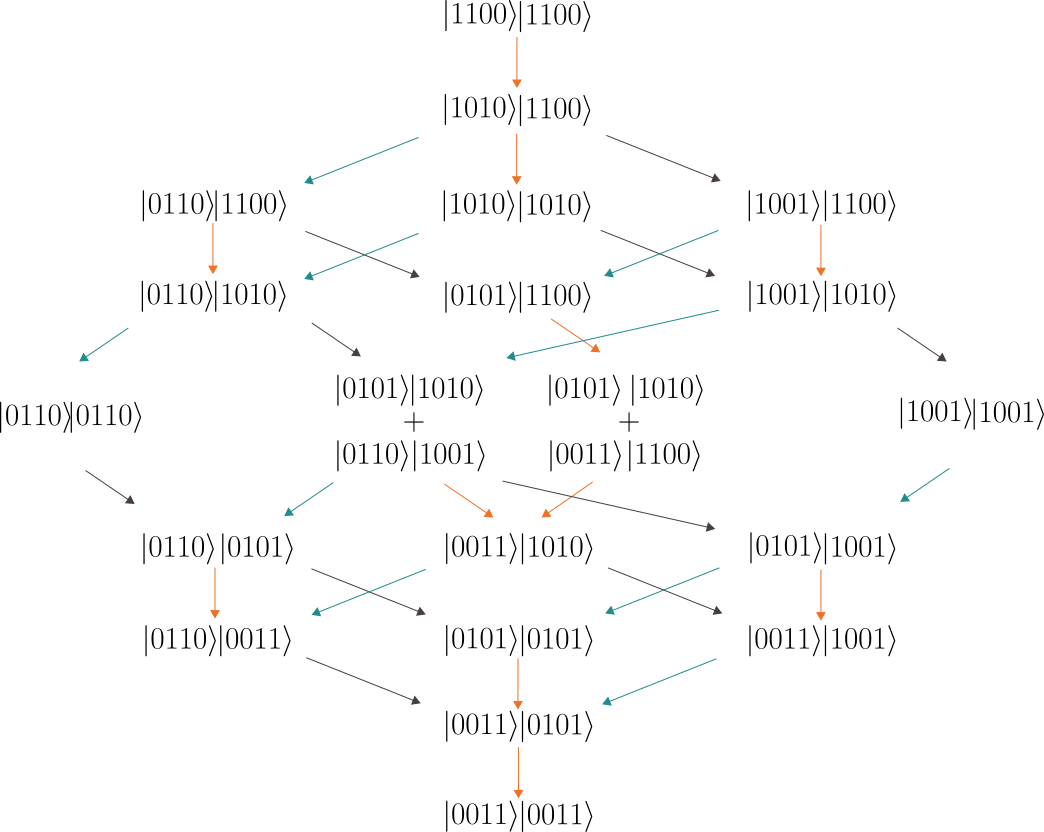
\includegraphics[scale=0.525]{img/hasse-diagram.png}
		\caption{The 20-dimensional irreducible symmetric subspace in ${\text 6_0 \otimes 6_0}$; The color of each arrow indicates the negative root \eqref{root-color} used to obtain the state. Every state is understood to be symmetrized.}
		\label{fig:hesse-diagram}
	\end{center}
\end{figure}
\begin{align}
\begin{split}
\ket{\beta} &= \frac{1}{\sqrt{6}} \Big( \ket{0101} \ket{1010}
	+ \ket{1010} \ket{0101}
	- \ket{0110} \ket{1001} \\
	&- \ket{1001} \ket{0110}
	- \ket{0011} \ket{1100}
	- \ket{1100} \ket{0011} \Big)
\end{split}
\end{align}
The singlets $\ket{1,0}$ and $\ket{35,0}$ are the linear combinations of $\ket{\alpha}$ and $\ket{\beta}$ annihilated by $a\dgg_1a\dgg_2 \otimes \id + \id \otimes a\dgg_1a\dgg_2$; they are
\begin{align}
\ket{\text 1,0} &= \frac{\ket{\alpha} + \sqrt{3} \ket{\beta} }{2}, &
\ket{\text 35,0} &= \frac{\sqrt{3} \ket{\alpha} - \ket{\beta} }{2}.
\end{align}
Note that $\ket{1,0}$, being simultaneously a $\gr{U}{4}$-singlet and the $\gr{Spin}{8}$-singlet, can also be obtained by the complex conjugation operator
\begin{align}
	\ket{1,0} &= -\id \otimes C_{8_+} \frac{1}{\sqrt{8}} \sum_j \ket{jj}.
\end{align}

Actually what we have found are singlets in $8_+ \otimes 8_+$, whereas the singlets in the Clebsch-Gordan coefficient $\Gamma_{\mu} = |\bra{\mu 0} (\ket{0000} \otimes \ket{0000})|$ are in $8_+ \otimes 8_+^*$. The two can be converted to one another by the complex conjugation operator:
\begin{align}
	\left| \prescript{}{8_+ \otimes 8_+^*}{}\!\!|\bra{\mu 0} (\ket{0000} \otimes \ket{0000}) \right|
		&= \left| \prescript{}{8_+ \otimes 8_+}{}\!\!\braket{\mu 0|\id \otimes C_{8_+}|0000} \otimes \ket{0000} \right| \\
		&= \left| \prescript{}{8_+ \otimes 8_+}{}\!\!|\bra{\mu 0} (\ket{0000} \otimes \ket{1111}) \right|.
\end{align}
Note that $\ket{0000}\ket{1111}$ is the highest weight state of $8_+ \otimes 8_+^*$ because $C_{8_+}$ swaps $a_j$ and $a\dgg_j$ ---that is, it swaps positive and negative roots of the Lie algebra. As a result,
\begin{align}\label{cg-coefficients}
	\Gamma_{\text 1}^2 &= \frac{1}{8}, & \Gamma_{\text 28}^2 &= \frac{1}{2}, & \Gamma_{\text 35}^2 &= \frac{3}{8}.
\end{align}


The spherical functions,
\begin{align}
	\rep_{\mu}(\Omega)_{00} &=
	\prescript{}{8_+\otimes 8_+}{}\!\!\braket{\mu 0|\rep_{8_+}\dgg(\Omega) \otimes U_{8_+}(\Omega)|\mu 0}_{8_+\otimes 8_+},
\end{align}
depend only the maximal abelian subgroup $A$ in the $KAK$ decomposition. Thus we can restrict $\rep_{8_+}$ to be
\begin{align}
\rep(\theta^+_{12},\theta^+_{34})_{8_+} &= \exp \left[ \frac{i}{2}(\theta^+_{12} Y^+_{12} + \theta^+_{34} Y^+_{34}) \right],
\end{align}
obtaining
\begin{align}
\rep_{1}(\theta^+_{12},\theta^+_{34})_{00} &= 1, \\
\rep_{28}(\theta^+_{12},\theta^+_{34})_{00} &= \frac{\cos(\theta^+_{12}) + \cos(\theta^+_{34})}{2}, \\
\rep_{35}(\theta^+_{12},\theta^+_{34})_{00} &= \frac{1+2\cos(\theta^+_{12}) \cos(\theta^+_{34})}{3}.
\end{align}
$(d_{\mu}/8)^{1/2} \rep_{\mu}(\Omega)_{00}$ are orthonormal functions with respect to the measure $d\Omega$ \eqref{measure}.

%------------------------------------
\subsection{Gaussian quasi-probability functions are negative}
%------------------------------------
The Q functions of Fermionic Gaussian states are
\begin{align}
\left| \braket{\Omega | \Omega'} \right|^2 &= \frac{1 + \cos\theta^+_{12} + \cos\theta^+_{34} + \cos\theta^+_{12}\cos\theta^+_{34}}{4},
\end{align}
which reduces to unity when $\Omega = \Omega'$. Alternatively, it is the product of spherical functions in the even spinor representation
\begin{align}
	U_8 (\theta_{12}^+) U_8 (\theta_{34}^+) &= \left( \frac{1 + \cos \theta_{12}^+}{2} \right) \left( \frac{1 + \cos \theta_{34}^+}{2} \right).
\end{align}
The quasi-probability function of the vacuum in the self-dual ($s=0$) representation is given by the formula
\begin{align}\label{brif-mann-wigner}
\mu_e (\Omega) &= \sum_{\mu} \Gamma_{\mu} \sqrt{ \frac{d_{\mu}}{d}} \rep_{\mu}(\Omega)_{00}.
\end{align}
The quasi-probability multiplied by the measure, depicted in Figure \ref{fig:wigner}, ends up taking negative values with an integrated negativity of $-0.47$. The measure vanishes on the line $\theta_{12}^+ = \theta_{34}^+$ and concentrates in the area where negativity occurs.
\begin{figure}[t]
	\begin{center}
	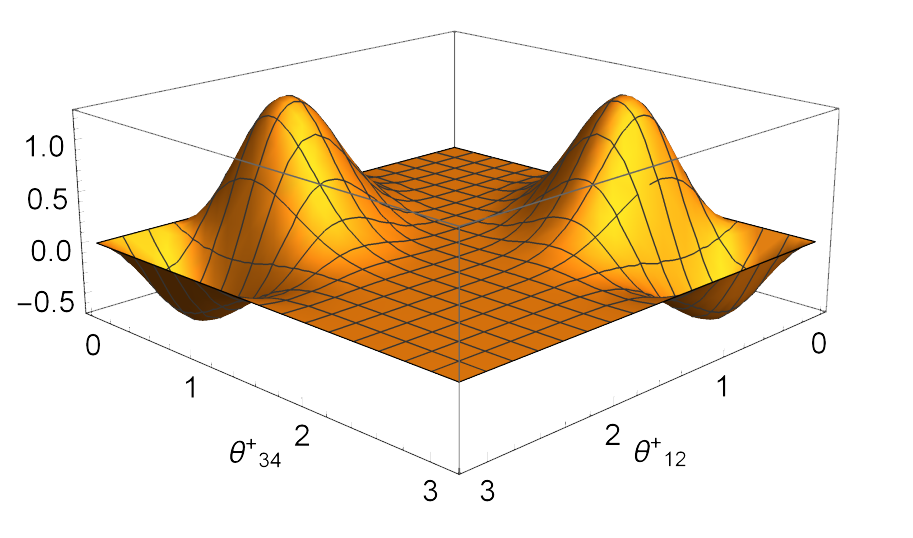
\includegraphics[scale=0.7]{img/SO-8-wigner.png}
	\caption{The Wigner function of pure fermionic Gaussian
		states, multiplied by the measure}
	\label{fig:wigner}
	\end{center}
\end{figure}

Let us briefly look at how the frame elements acquire negative eigenvalues. The frame is given by the formula
\begin{align}
F(\Omega,s) &= \sum_{\mu} \frac{1}{\Gamma_{\mu}^{1+s}} \left( \frac{d_{\mu}}{d} \right)^{(3+s)/2}
\int d\Omega'\,\rep_{\mu}(\Omega^{-1}\Omega')_{00} \ketbra{\Omega'}{\Omega'} \\
	&= \sum_{\mu} \left( \frac{d_{\mu}}{d\Gamma_{\mu}^2} \right)^{(1+s)/2} \frac{d_{\mu}}{d}
	\int d\Omega'\,\rep_{\mu}(\Omega^{-1}\Omega')_{00} \ketbra{\Omega'}{\Omega'}
\end{align}
By construction, any frame element can be obtained from another by the group action, so we can consider the frame element at $\Omega = 0$ for simplicity. In this case, it turns out that the integrals can be written in terms of $P_k$, the projection operators onto the $k$-particle sectors, as follows:
\begin{align}
	\int d\Omega\,\ketbra{\Omega}{\Omega} &= \id, \\
	\int d\Omega\,\rep_{28}(\Omega)_{00} \ketbra{\Omega}{\Omega} &= \frac{8}{28}\frac{P_0 - P_4}{2}, \\
	\int d\Omega\,\rep_{35}(\Omega)_{00} \ketbra{\Omega}{\Omega} &= \frac{8}{35} \left[ \frac{3}{8}(P_0 + P_4) - \frac{P_2}{8} \right].
\end{align}
Putting these together gives us
\begin{align}
F(0,s) &=	\frac{\id}{8}
	+ 7^{(1+s)/2} \frac{P_0 - P_4}{2}
	+ \left( \frac{35}{3} \right)^{(1+s)/2} \left[ \frac{3}{8}(P_0 + P_4) - \frac{P_2}{8} \right].
\end{align}
Setting $s = -1$, $P_2$ in the first and last term cancel exactly to reproduce the vacuum projection operator:
\begin{align}
F(0,-1) &= \left( \frac{1}{8} + \frac{1}{2} + \frac{3}{8} \right) P_0 + \left( \frac{1}{8} - \frac{1}{2} + \frac{3}{8} \right) P_4 = P_0.
\end{align}
As soon as $s>-1$, the negative contribution of $P_2$ in the last term wins and each frame element ceases to be a positive operator. For the self-dual frame $s=0$,
\begin{align}
F(0,0) &= \left( \frac{1}{8} + \frac{\sqrt{7}}{2} + \frac{\sqrt{105}}{8} \right) P_0 +  \left( \frac{1}{8} - \frac{\sqrt{7}}{2} + \frac{\sqrt{105}}{8} \right) P_4 +  \left( 1 - \sqrt{\frac{35}{3}} \right) \frac{P_2}{8} \\
&\approx 2.72 P_0 + 0.08 P_4 - 0.30 P_2,
\end{align}

%Thus,
%\begin{align}
%	F(\Omega,1) &= U(\Omega^{-1}) P_0 U(\Omega) \left( \frac{1}{8} + \frac{\sqrt{7}}{2} + \frac{\sqrt{105}}{8} \right) + P_4 \left( \frac{1}{8} - \frac{\sqrt{7}}{2} + \frac{\sqrt{105}}{8} \right) + \frac{P_2}{8} \left( 1 - \sqrt{\frac{35}{3}} \right)
%\end{align} 